
%(BEGIN_QUESTION)
% Copyright 2013, Tony R. Kuphaldt, released under the Creative Commons Attribution License (v 1.0)
% This means you may do almost anything with this work of mine, so long as you give me proper credit

This solar collector temperature control system has a problem.  The indicating controller (TIC) shows a temperature much colder than ambient, even though the temperature gauge (TG) registers 185 $^{o}$F and the controller setpoint is set to 132 $^{o}$F.  A voltmeter connected between the loop power terminals on the temperature transmitter registers 23.0 VDC:

$$\includegraphics[width=15.5cm]{i03365x01.eps}$$

Identify the likelihood of each specified fault for this circuit.  Consider each fault one at a time (i.e. no coincidental faults), determining whether or not each fault could independently account for {\it all} measurements and symptoms in this circuit.

% No blank lines allowed between lines of an \halign structure!
% I use comments (%) instead, so that TeX doesn't choke.

$$\vbox{\offinterlineskip
\halign{\strut
\vrule \quad\hfil # \ \hfil & 
\vrule \quad\hfil # \ \hfil & 
\vrule \quad\hfil # \ \hfil \vrule \cr
\noalign{\hrule}
%
% First row
{\bf Fault} & {\bf Possible} & {\bf Impossible} \cr
%
\noalign{\hrule}
%
% Another row
250 ohm resistor at controller input failed open &  &  \cr
%
\noalign{\hrule}
%
% Another row
Cable between temperature transmitter and controller failed open &  &  \cr
%
\noalign{\hrule}
%
% Another row
Cable between temperature transmitter and controller failed shorted &  &  \cr
%
\noalign{\hrule}
%
% Another row
Temperature transmitter failed with low signal &  &  \cr
%
\noalign{\hrule}
%
% Another row
Cable between controller and VSD failed open &  &  \cr
%
\noalign{\hrule}
%
% Another row
Cable between controller and VSD failed shorted &  &  \cr
%
\noalign{\hrule}
%
% Another row
DC fan motor windings failed open &  &  \cr
%
\noalign{\hrule}
} % End of \halign 
}$$ % End of \vbox

\underbar{file i03365}
%(END_QUESTION)





%(BEGIN_ANSWER)

% No blank lines allowed between lines of an \halign structure!
% I use comments (%) instead, so that TeX doesn't choke.

$$\vbox{\offinterlineskip
\halign{\strut
\vrule \quad\hfil # \ \hfil & 
\vrule \quad\hfil # \ \hfil & 
\vrule \quad\hfil # \ \hfil \vrule \cr
\noalign{\hrule}
%
% First row
{\bf Fault} & {\bf Possible} & {\bf Impossible} \cr
%
\noalign{\hrule}
%
% Another row
250 ohm resistor at controller input failed open &  & $\surd$ \cr
%
\noalign{\hrule}
%
% Another row
Cable between temperature transmitter and controller failed open &  & $\surd$ \cr
%
\noalign{\hrule}
%
% Another row
Cable between temperature transmitter and controller failed shorted &  & $\surd$ \cr
%
\noalign{\hrule}
%
% Another row
Temperature transmitter failed with low signal & $\surd$ &  \cr
%
\noalign{\hrule}
%
% Another row
Cable between controller and VSD failed open &  & $\surd$ \cr
%
\noalign{\hrule}
%
% Another row
Cable between controller and VSD failed shorted &  & $\surd$ \cr
%
\noalign{\hrule}
%
% Another row
DC fan motor windings failed open &  & $\surd$ \cr
%
\noalign{\hrule}
} % End of \halign 
}$$ % End of \vbox


%(END_ANSWER)





%(BEGIN_NOTES)

{\bf This question is intended for exams only and not worksheets!}.

%(END_NOTES)


